\documentclass[11pt]{article}
\usepackage{amssymb}
\usepackage{amsthm}
\usepackage{enumitem}
\usepackage{amsmath}
\usepackage{bm}
\usepackage{adjustbox}
\usepackage{mathrsfs}
\usepackage{graphicx}
\usepackage{siunitx}
\usepackage[mathscr]{euscript}

\title{\textbf{Solved selected problems of Classical Mechanics - Taylor}}
\author{Franco Zacco}
\date{}

\addtolength{\topmargin}{-3cm}
\addtolength{\textheight}{3cm}

\newcommand{\hatr}{\bm{\hat{r}}}
\newcommand{\hatx}{\bm{\hat{x}}}
\newcommand{\haty}{\bm{\hat{y}}}
\newcommand{\hatz}{\bm{\hat{z}}}
\newcommand{\hatth}{\bm{\hat{\theta}}}
\newcommand{\hatphi}{\bm{\hat{\phi}}}
\newcommand{\hatrho}{\bm{\hat{\rho}}}
\renewcommand*{\proofname}{Solution}

\begin{document}
\maketitle
\thispagestyle{empty}

\section*{Chapter 1 - Newton's laws of Motion}

	\begin{proof}{\textbf{1.10}}
        The cartesian components x and y for the vector $r$ are 
        $$x = R \cos{\theta} \quad\quad y = R \sin{\theta}$$
        we also know that $\theta = \omega t$
        so we have that
        \begin{align*}
            \bm{r} &= \hatx R \cos{\theta}  + \haty R \sin{\theta} \\
                   &= \hatx R \cos{\omega t} + \haty R \sin{\omega t}
        \end{align*}
        To find the particle's velocity and acceleration we must differetiate
        the $\bm{r}$ equation with respect to time.\\
        For the velocity we have that 
        \begin{align*}
            \frac{d\bm{r}}{dt} &= \frac{d}{dt}(\hatx R \cos{\omega t}  + \haty R \sin{\omega t}) \\
                        \bm{v} &= - \hatx R \omega \sin{\omega t} + \haty R \omega \cos{\omega t}
        \end{align*}
        For the acceleration we need to differentiate the velocity again 
        \begin{align*}
            \frac{d\bm{v}}{dt} &= \frac{d}{dt}(- \hatx R \omega \sin{\omega t} + \haty R \omega \cos{\omega t}) \\
                        \bm{a} &= - \hatx R \omega^2 \cos{\omega t} - \haty R \omega^2 \sin{\omega t}
        \end{align*}
        as noticed the direction of the acceleration is oposite to $\bm{r}$.
        Finally, the magnitude of the acceleration is
        \begin{align*}
            |\bm{a}| &= \sqrt{(-R \omega^2 \cos{\omega t})^2 + (-R \omega^2 \sin{\omega t})^2} \\
                     &= \sqrt{R^2 \omega^4(\cos^2{\omega t} + \sin^2{\omega t})} \\
                     &= R \omega^2
        \end{align*}
        \end{proof}
\cleardoublepage
        \begin{proof}{\textbf{1.11}}
            Given that the position of the particle is given by
            $$\bm{r}(t) = \hatx b \cos{\omega t} + \haty c \sin{\omega t}$$
            Then the cartesian coordinates for the particle are
            $x = b \cos{\omega t}$ and $y = c \sin{\omega t}$
            
            We can derive from the identity $\cos^2{\omega t} + \sin^2{\omega t} = 1$
            the equation that involves both cartesian coordinates as follows.
            \begin{align*}
                \cos^2{\omega t} + \sin^2{\omega t} &= 1 \\
                \frac{b^2}{b^2}\cos^2{\omega t} + \frac{c^2}{c^2}\sin^2{\omega t} &= 1 \\
                \frac{x^2}{b^2} + \frac{y^2}{c^2} &= 1
            \end{align*}
            Which is the equation for an ellipse centered at the origin.
        \end{proof}
        \begin{proof}{\textbf{1.12}}
            In this case, the particle in addition to being rotating around an
            ellipse trajectory as we already know from the last problem is also
            moving in the positive direction around the $z$-axis so the
            resultant trajectory is a helicoid centered around $z$-axis.
        \end{proof}
        \begin{proof}{\textbf{1.26}}
            \begin{itemize}
            \item[(a)] Given a reference frame $\mathscr{S}$ where the x-axis
            point east and y-axis point north, if we kick a frictionless puck
            due north, from this reference frame, there is no x-axis movement
            for the puck and it moves to north with constant velocity, then
            the coordinates for the puck are
            $$x = 0 \quad\quad y = vt$$
            where $v$ is the constant velocity at which the puck is moving.
            \item[(b)] In a reference frame $\mathscr{S'}$ which is moving
            with constant velocity $v'$ due east with respect to
            $\mathscr{S}$ the puck movement seen from $\mathscr{S'}$ has an
            added movement in the $-x$ direction since $\mathscr{S'}$ is moving
            away from the puck so the coordinates for the puck seen from
            $\mathscr{S'}$ are 
            $$x' = -v't \quad\quad y' = vt$$
            this means that the puck has a trajectory given by $y' = -v/v' x'$
            which is a line with a negative slope that passes through the origin.
            \item[(c)] Lastly the reference frame $\mathscr{S''}$ is moving
            with constant acceleration due east with respect to $\mathscr{S}$
            so the puck movement seen from $\mathscr{S''}$ has an added
            movement in the $-x$ direction since $\mathscr{S''}$ is moving
            away from the puck, therefore the coordinates for the puck seen from
            $\mathscr{S''}$ are
            $$x'' = -(v''t + \frac{1}{2}a''t^2) \quad\quad y'' = vt$$
            where $v''$ and $a''$ are the velocity and acceleration of
            $\mathscr{S''}$ respectively. 
            \end{itemize}
            Since $\mathscr{S}$ and $\mathscr{S'}$ are not accelerating they
            are inertial reference frames, which is not the case for
            $\mathscr{S''}$.
        \end{proof}
        \begin{proof}{\textbf{1.27}}
            The puck path observed by someone sitting at rest at the origin of
            the turntable is a spiral that grows indefinitely as the puck
            continues its path to infinity. 
        \end{proof}
        \begin{proof}{\textbf{1.30}}
            The total momentum of the system before the collision is given by
            $$\bm{P} = m_1 \bm{v} + m_2 0 = m_1 \bm{v}$$
            but after the collision the total momentum is given by
            $$\bm{P} = m_1 \bm{v'} + m_2 \bm{v'}$$
            since there is no external forces, then the total momentum of the
            system is constant, therefore
            \begin{align*}
                m_1 \bm{v'} + m_2 \bm{v'} &= m_1 \bm{v}\\
                       \bm{v'}(m_1 + m_2) &= m_1 \bm{v} \\
                                  \bm{v'} &= \frac{m_1}{m_1 + m_2}\bm{v}
            \end{align*}
        \end{proof}
        \begin{proof}{\textbf{1.40}}
            \begin{itemize}
            \item [(a)] According to the Newton's second Law we have that
            $\bm{F} = m\bm{\ddot{r}}$ or if we write it in cartesian coordinates
            for two dimensions then 
            $$F_x\hatx + F_y \haty = m\ddot{x} \hatx + m\ddot{y} \haty$$
            given that the only force is the gravitational force and is in the
            y-direction we have that
            $$m\ddot{x} = 0\quad \quad m\ddot{y} = -mg$$
            therefore integrating both equations we have that
            \begin{align*}
                \dot{x} &= \int{0~dt} \\
                        &= 0 + v_{0x} \\
                      x &= \int{v_{0x}~dt} \\
                        &= v_{0x}t + x_0 \\
                        &= v_{0x}t
            \end{align*}
            where $v_{0x}$ and $x_0$ are the initial velocity and position of
            the ball in the $x$-direction, note that $x_0 = 0$.
            Also we have that $v_{0x} = v_0 \cos{\theta}$ so the final equation
            is $$x = v_0 t \cos{\theta}$$ 
            In the same way for the $y$-direction we have that
            \begin{align*}
                \dot{y} &= \int{-g~dt} \\
                        &= v_{0y} - gt \\
                      y &= \int{v_{0y} - gt~dt} \\
                        &= y_0 + v_{0y}t - g \frac{t^2}{2}\\
                        &= v_{0y}t - g \frac{t^2}{2}
            \end{align*}
            As we know from the $x$-direction $v_{0y} = v_0 \sin{\theta}$ so the final equation
            becomes $$y = v_{0}t\sin{\theta} - g \frac{t^2}{2}$$
            \item [(b)] We write the $r^2$ (the magnitude of $\bm{r}$ squared)
            as
            \begin{align*}
                r^2 &= (v_0 t\cos{\theta})^2 + \left(v_0 t\sin{\theta} - g \frac{t^2}{2}\right)^2 \\
                    &= (v_0 t\cos{\theta})^2 + (v_0 t\sin{\theta})^2 - 2 g
                    \frac{t^2}{2} v_0 t\sin{\theta} + \left(-g \frac{t^2}{2}\right)^2 \\
                    &= (v_0t)^2(\cos^2{\theta} + \sin^2{\theta}) - g v_0 t^3
                    \sin{\theta} + \left(-g \frac{t^2}{2}\right)^2 \\
                    &= (v_0t)^2 - g v_0t^3 \sin{\theta} +
                    \left(-g \frac{t^2}{2}\right)^2
            \end{align*}
            To check whether a function increases or decreases we need to
            analyze the equation's derivative. Then
            \begin{align*}
                \dot{r^2} &= 2 v_0^2 t - 3g v_0 t^2 \sin{\theta} + g^2 t^3 
            \end{align*}
            What we want is that $2 v_0^2t - 3g v_0 t^2 \sin{\theta} + g^2 t^3 > 0$.
            The minimum of $\dot{r^2}$ can be found by differentiating this
            equation again and solving for $\ddot{r^2} = 0$, so
            $$2v_0^2 - 6gv_0t\sin{\theta} + 3g^2t^2 = 0$$
            \begin{align*}
                t_{min} &= \frac{6gv_0\sin{\theta} \pm \sqrt{(-6gv_0 \sin{\theta})^2
                        - 24g^2v_02}}{6g^2} \\
                        &= \frac{6gv_0\sin{\theta} \pm \sqrt{36g^2v_0^2 \sin^2{\theta}
                        - 24g^2v_02}}{6g^2} \\
                        &= \frac{6gv_0\sin{\theta} \pm 6gv_0\sqrt{\sin^2{\theta}
                        - 24/36}}{6g^2} \\
                        &= \frac{v_0}{g}(\sin{\theta} \pm \sqrt{\sin^2{\theta}
                        - 6/9}) \\
                \end{align*}
            The next step would be to write $\dot{r^2}$ valued at $t_{min}$ and
            find where this expression is $>0$ to determine the value for
            $\theta$.            
        \end{itemize}
    \end{proof}
    \begin{proof}{\textbf{1.41}}
        The Newton's second law in polar coordinates are
        $$F_r = m(\ddot{r} - r \dot{\phi}^2)$$
        $$F_{\phi} = m(r \ddot{\phi} + 2\dot{r}\dot{\phi})$$
        where in this case $\dot{\phi} = \omega$ and since $\omega$ is
        constant $\ddot{\phi} = 0$ also $r=R$ which is also constant then
        $\dot{r} = \ddot{r} = 0$, therefore
        \begin{align*}
            F_r &= -mR\omega^2 \quad\quad F_{\phi} = 0
        \end{align*}
        Since the tension is the only force in the $r$ direction we have
        that
        $$T = -mR\omega^2$$
    \end{proof}
    \begin{proof}{\textbf{1.46}}
        \begin{itemize}
            \item[(a)] For an observer on the ground in a reference frame
            $\mathscr{S}$ with its origin $O$ at the center of the turntable
            the puck will have polar coordinates given by
            $$\bm{\phi} = 0$$
            $$\bm{r} = (R - vt) \hatr $$
            where $R$ is the radius of the turntable and $v$ the velocity of
            the puck.
            \item[(b)] In the case that the observer is fixed to the turntable
            with its origin $O$ at the center of the turntable the puck will
            have the same $\bm{r}$ polar coordinate but now $\bm{\phi}$ is
            changing according to the rotation of the reference frame therefore 
            $$\bm{\phi'} = \omega t \hatphi $$
            $$\bm{r'} = (R - vt) \hatr $$
            where $\omega$ is the angular velocity of the turntable.
            This is not an inertial reference frame since it's rotating.
        \end{itemize}
    \end{proof}
\cleardoublepage
    \begin{proof}{\textbf{1.47}}
        \begin{itemize}
            \item[(a)] The expressions for $\rho$, $\phi$, and $z$ in terms of
            $x$, $y$, and $z$ are
            $$\rho = \sqrt{x^2 + y^2}$$
            $$\phi = \arctan{(y/x)}$$
            $$z = z$$
            In words, $\rho$ is the distance to $P'$ from the origin, where
            $P'$ is the projection of $P$ to the plane $(x,y,0)$.\\
            The use of $r$ to name $\rho$ in this case is unfortunate since we
            are naming $r$ as the magnitude of the vector $\bm{r}$ which is the
            distance to $P$ from the origin.
            \item[(b)] The unit vector $\hatrho$ is the same unit vector we
            defined previously for two dimensions problems as $\hatr$ and the same
            thing happening with $\hatphi$. In the case of $\hatz$ is a unit
            vector that points in the direction of the $z$ cartesian coordinate.\\
            The position vector in this case is given by
            $$\bm{r} = \rho\hatrho + z \hatz$$
            \item[(c)] Given that $\hatz$ is the same unit vector as in
            cartesian coordinates then $d\hatz/dt = 0$ also using the result
            we obtained for $d\hatr/dt = d\hatrho/dt$ and $d\hatphi/dt$ we get
            that
            \begin{align*}
                \dot{\bm{r}} = \bm{v} &= \left(
                    \dot{\rho}\hatrho + \rho\frac{d\hatrho}{dt}
                \right) + \dot{z}\hatz \\
                             &= \dot{\rho}\hatrho + \rho\dot{\phi}\hatphi
                + \dot{z}\hatz
            \end{align*}
            Then
            \begin{align*}
                \ddot{\bm{r}} = \bm{a} &= \left(
                    \ddot{\rho}\hatrho + \dot{\rho}\frac{d\hatrho}{dt}
                \right) +
                \left(
                    (\dot{\rho}\dot{\phi} + \rho \ddot{\phi})\hatphi +
                    \rho\dot{\phi}\frac{d\hatphi}{dt}
                \right) + \ddot{z}\hatz \\
                             &= (\ddot{\rho} - \rho\dot{\phi}^2)\hatrho +
                (\rho\ddot{\phi} + 2\dot{\rho}\dot{\phi})\hatphi + \ddot{z}\hatz
            \end{align*}
        \end{itemize}
    \end{proof}
\cleardoublepage
    \begin{proof}{\textbf{1.48}}
        The projection of $\hatrho$ to the x-axis is given by $\cos{\phi}$ and
        the projection to the y-axis is given by $\sin{\phi}$ then
        $$\hatrho = \hatx \cos{\phi} + \haty \sin{\phi}$$
        since $\hatphi$ is perpendicular to $\hatrho$ then
        $$\hatphi = - \hatx \sin{\phi} + \haty \cos{\phi}$$
        and since $\hatz$ is the same as the one used in cartesian coordinates
        $$\hatz = \hatz$$
        The derivatives of the above equations given that $d\hatx/dt = 0$,
        $d\haty/dt = 0$, and $d\hatz/dt = 0$ are
        \begin{align*}
            \frac{d\hatrho}{dt} &= (
                \frac{d\hatx}{dt} \cos{\phi} - \hatx \dot{\phi}\sin{\phi}
            ) + (
                \frac{d\haty}{dt} \sin{\phi} + \haty \dot{\phi}\cos{\phi}
            ) \\
                                &= - \hatx \dot{\phi}\sin{\phi} + \haty \dot{\phi}\cos{\phi} \\
                                &= \dot{\phi} (-\hatx\sin{\phi} + \haty\cos{\phi}) \\
                                &= \dot{\phi} \hatphi
        \end{align*}
        \begin{align*}
            \frac{d\hatphi}{dt} &= -(
                \frac{d\hatx}{dt} \sin{\phi} + \hatx \dot{\phi}\cos{\phi}
            ) + (
                \frac{d\haty}{dt} \cos{\phi} - \haty \dot{\phi}\sin{\phi}
            ) \\
                                &= - \hatx \dot{\phi}\cos{\phi} - \haty \dot{\phi}\sin{\phi} \\
                                &= -\dot{\phi}(\hatx\cos{\phi} + \haty\sin{\phi}) \\
                                &= -\dot{\phi}\hatrho \\ \\
              \frac{d\hatz}{dt} &= 0
        \end{align*}        
    \end{proof}
    \begin{proof}{\textbf{1.49}}
        Newton's second law equations in cylindrical coordtinates are
        \begin{align*}
            F_{\phi} &= m(\rho\ddot{\phi} + 2\dot{\rho}\dot{\phi}) \\
            F_{\rho} &= m(\ddot{\rho} - \rho\dot{\phi}^2) \\
            F_{z} &= m\ddot{z}
        \end{align*}
        Given that the puck is fixed to a certain $\rho=R$ then
        $\dot{\rho}=\ddot{\rho}=0$ also since the gravitational force is in the
        $z$ direction, we have that
        \begin{align}
            0 &= mR\ddot{\phi} \\
            N_1 - N_2 = N &= - mR\dot{\phi}^2 \\
          -mg &= m\ddot{z}
        \end{align}
        where $N_1$ and $N_2$ are the two normal forces exerted by the two 
        cylinders, we named the difference between them $N$.\\
        Integrating the equation (1) we have that
        \begin{align*}
            \dot{\phi} = \omega &= \int 0 dt \\
                      &= 0 + \omega_0
        \end{align*}
        where $\omega_0$ is the angular velocity and integrating
        again we have that
        \begin{align*}
            \phi &= \int \omega_0dt \\
                 &= \omega_0t + \phi_0
        \end{align*}
        Then integrating the equation (3), we have that
        \begin{align*}
            \dot{z} = v_{z} &= \int-g dt \\
                            &= -gt + v_{z0}
        \end{align*}
        and integrating again we have that
        \begin{align*}
            z &= \int{(-gt + v_{z0})dt} \\
              &= -g\frac{t^2}{2} + v_{z0}t +z_0
        \end{align*}
        Then the movement in the $z$-direction is as a free falling object
        and in the $\phi$-direction is a rotation with constant angular velocity.
        Therefore the final trajectory is a downward helix.
    \end{proof}
    \begin{proof}{\textbf{1.50}}
        We can transform the 2nd order equation
        $$\ddot{\phi} = - \frac{g}{R}\sin{\phi}$$
        into two 1st order equation as
        \begin{align*}
            \dot{\phi} &= \omega \\
            \dot{\omega} &=  - \frac{g}{R}\sin{\phi}
        \end{align*}
        Solving this system of equations with the improved Euler method we get
        the following graph.\\
        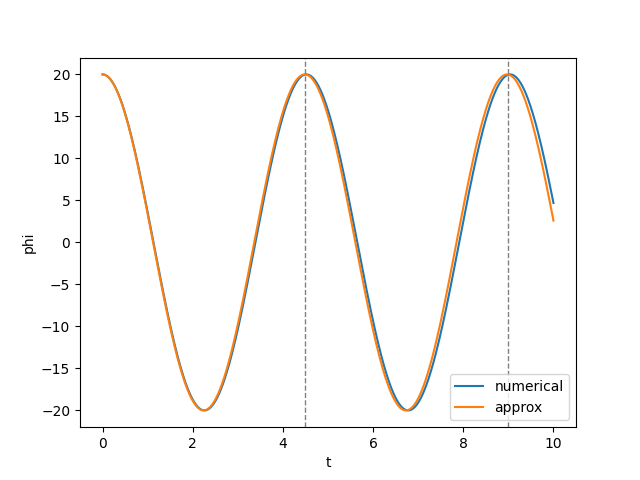
\includegraphics{taylor-1.50.png}
    \end{proof}
\cleardoublepage
    \begin{proof}{\textbf{1.51}}\\
        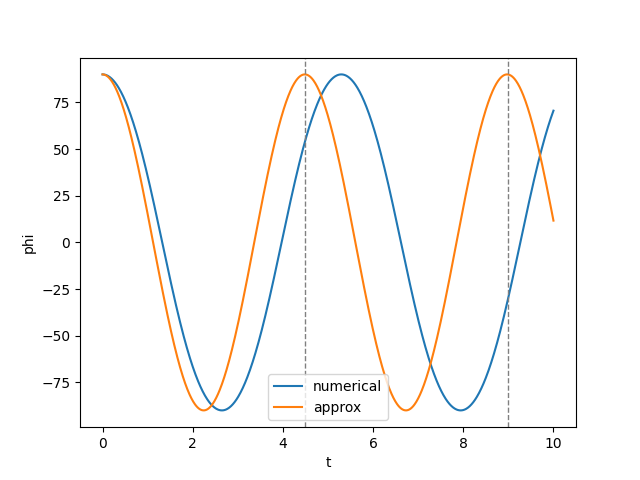
\includegraphics{taylor-1.51.png}   
    \end{proof}

\end{document}























